\subsubsection{Zweite Phase}
\label{bpr:algorithmus:phase2}

Zu Beginn dieser Phase des Algorithmus existiert bereits ein (noch nicht fertig sortiertes) Suffix-Array \sa, welches nun rekursiv sortiert werden soll. Die aktuelle Einteilung der Suffixe in Buckets ist über den Bucket Pointer \bptr gegeben, aus dem abgelesen werden kann, ob sich zwei Suffixe im gleichen oder in verschiedenen Buckets befinden. Das Array \bkt, welches in der ersten Phase des Algorithmus erstellt wurde, um die initiale Zuteilung festzulegen, wird im weiteren Verlauf nicht mehr verwendet.\par
Die Sortierung erfolgt rekursiv für jeden Bucket im Suffix-Array. Da die einzelnen Buckets untereinander zu jedem Zeitpunkt bereits sortiert sind, muss der Sortiervorgang in jedem Rekursionsschritt nur innerhalb des jeweiligen Buckets stattfinden. Da es für effizientes Sortieren aber erforderlich ist, zwei Suffixe mit konstantem Aufwand vergleichen zu können, werden wir zunächst sehen, anhand welcher Kriterien wir Suffixe effizient vergleichen können.
\begin{figure}[ht]
	\resizebox{\textwidth}{!}{
			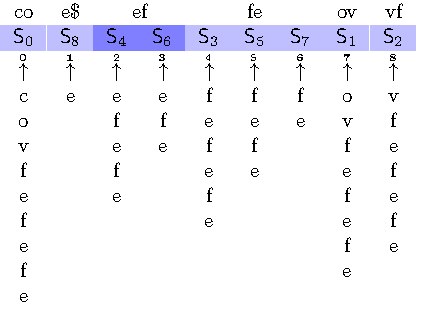
\includegraphics{kapitel/saca_algorithmen/bpr/algorithmus/phase2/buckets_initial_compare/image.pdf}
			\hspace{1em}
			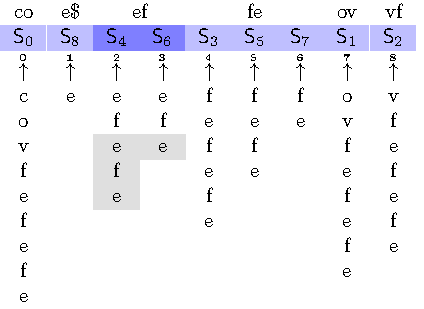
\includegraphics{kapitel/saca_algorithmen/bpr/algorithmus/phase2/buckets_initial_compare_highlight/image.pdf}
	}
	\caption{Vergleich zweier Suffixe innerhalb eines Buckets}
	\label{fig:inner_bucket}
\end{figure}
Am bereits zuvor eingeführten Beispiel beginnen wir, den Bucket \bucket{\textup{ef}} zu sortieren (Abbildung~\ref{fig:inner_bucket}). Der Bucket beinhaltet die Suffixe \suffix{4} und \suffix{6}, welche nach dem Sortierschritt in Phase 1 einen gemeinsamen Präfix der Länge \(d = 2\) haben. Da die Sortierung der Suffixe lexikographisch erfolgen soll, können gemeinsame Präfixe ignoriert werden, ohne die Korrektheit der Sortierung zu beeinflussen. 
Für Suffixe \(\suffix{i}, \suffix{j}\) mit \(i, j \in \mathsf{b}\) gibt der Level des Buckets \(\mathsf{b}\) eine untere Schranke für \offset an. Im Falle des Beispiels genügt es also, die Suffixe \(\suffix{4+2} = \suffix{6}\) und \(\suffix{6+2} = \suffix{8}\) zu vergleichen (Abbildung~\ref{fig:buckets_compare_and_sort}, oben links). Da selbstverständlich Suffixe der Suffixe von \inputtext auch selbst Suffixe von \inputtext sind, befinden sich auch diese in \sa. Falls  sich \(\suffix{i+\offset}\) und \(\suffix{j+\offset}\) bereits in verschiedenen Buckets befinden, ist das lexikographische Verhältnis dieser beiden Suffixe bereits bekannt. Um dies herauszufinden, werden die Bucket Pointer der entsprechenden Suffixe verglichen. Diese befinden sich im Array \bptr, welches bereits in Phase 1 initialisiert wurde und beinhalten einen Verweis auf die rechte Grenze des Buckets, in dem sich der jeweilige Suffix befindet.\par
\begin{figure}[ht]
	\resizebox{\textwidth}{!}{
		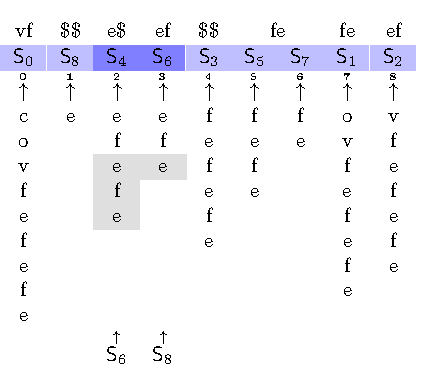
\includegraphics[valign=t]{kapitel/saca_algorithmen/bpr/algorithmus/phase2/buckets_initial_compare_highlight_label/image.pdf}
		\hspace{1em}
		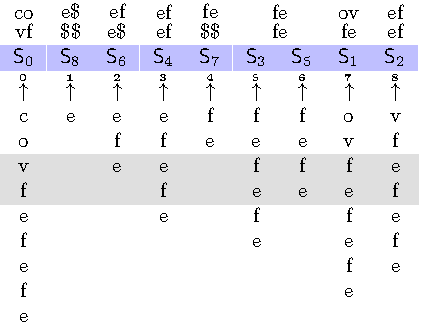
\includegraphics[valign=t]{kapitel/saca_algorithmen/bpr/algorithmus/phase2/buckets_updated/image.pdf}
	}\vspace{1ex}
	\resizebox{\textwidth}{!}{
		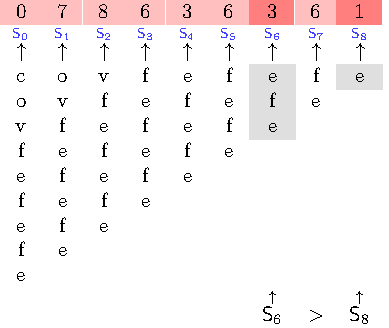
\includegraphics[valign=t]{kapitel/saca_algorithmen/bpr/algorithmus/phase2/bptr_initial_highlighted/image.pdf}
		\hspace{1em}
		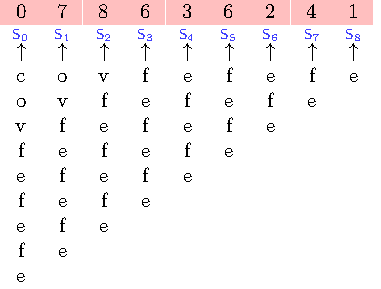
\includegraphics[valign=t]{kapitel/saca_algorithmen/bpr/algorithmus/phase2/bptr_updated/image.pdf}
	}
	\caption[Buckets sowie Bucket-Pointer vor und nach der ersten Verfeinerung]{Buckets (oben) sowie Bucket-Pointer (unten) vor und nach der ersten Verfeinerung. Es ist gut zu erkennen, dass bereits bei einer Rekursionstiefe von 1 nur noch ein nicht eindeutig sortierter Bucket existiert.}
	\label{fig:buckets_compare_and_sort}
\end{figure}
Abbildung~\ref{fig:buckets_compare_and_sort} (unten links) zeigt die Bucket Pointer der Suffixe \(\suffix{6}\) (Bucket \(\bucket{\textup{ef}}\) mit rechter Grenze an Index 3 in \sa) und \(\suffix{8}\) (Bucket \(\bucket{\textup{e\$}}\) mit rechter Grenze an Index 1 in \sa). Aus einem einfachen Vergleich dieser Bucket Pointer geht hervor, dass \(\suffix{8}\) lexikographisch kleiner ist als \(\suffix{6}\). Mithilfe von \cref{lemma:common_prefix} kann daraus geschlossen werden, dass auch \(\suffix{6}\) lexikographisch kleiner ist als \(\suffix{4}\). Ein solcher Vergleich kann durch zwei Zugriffe auf das Array \bptr in konstanter Zeit durchgeführt werden. Zur Veranschaulichung zeigt Abbildung~\ref{fig:buckets_compare_and_sort} (rechts) den Zustand von \sa und \bptr, wenn in \sa nur noch Level-4-Buckets enthalten sind. Nachdem ein Verfeinerungsschritt in einem Bucket \(\bucket{\textup{p}} = [l,r]\) in kleinere Buckets durchgeführt wurde, müssen außerdem die zugehörigen Bucket-Pointer im Array \bptr angepasst werden. Dazu wird der Bucket \(\bucket{\textup{p}}\) von rechts nach links durchlaufen, wobei für jeden darin enthaltenen Suffix \(\sa[i], l \leq i \leq r,\) der Sortiertschlüssel \(\bptr[\sa[i]+\offset]\) abgefragt. Es wird dann zwischen zwei Fällen unterschieden:

\begin{description}
	\item[Fall 1:]\(\bptr[\sa[i-1]+\offset] = \bptr[\sa[i]+\offset]\) \\
		Die Sortierschlüssel der Suffixe \(\sa[i-1]\) und \(\sa[i]\) sind identisch. Daher konnte in diesem Schritt keine echte Sortierung dieser beiden Suffixe vorgenommen werden. Deshalb befinden sie sich nach wie vor in einem gemeinsamen Bucket und \(\bptr[\sa[i-1]]\) wird auf \(\bptr[\sa[i]]\) gesetzt.
	\item[Fall 2:] \(\bptr[\sa[i-1]+\offset] \neq \bptr[\sa[i]+\offset]\) \\
		Die Sortierschlüssel der Suffixe \(\sa[i-1]\) und \(\sa[i]\) unterscheiden sich. Die Suffixe konnten also sortiert werden und befinden sich nach der Verfeinerung in unterschiedlichen Buckets. \(\sa[i-1]\) ist das erste Element von rechts in dem neu beginnenden Bucket. Folglich wird \(\bptr[\sa[i-1]]\) auf \(i-1\) gesetzt.
\end{description}

\noindent Nachdem die Bucket-Pointer aktualisiert wurden, ist der Sortiervorgang für \(\bucket{\textup{p}}\) abgeschlossen und es kann rekursiv fortgefahren werden. Das fertig sortierte Suffix-Array (links), welches nach Abschluss der Sortierung nur noch Buckets der Größe 1 enthält, sowie die dazugehörigen Bucket-Pointer (rechts) sind in Abbildung~\ref{fig:buckets_final} zu sehen.\par\smallskip
\begin{figure}[ht]
	\resizebox{\textwidth}{!}{
		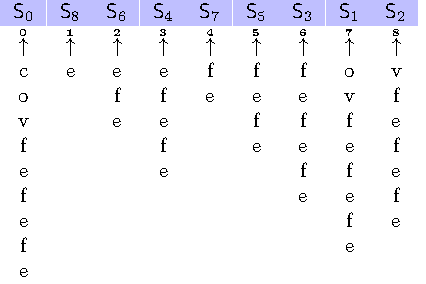
\includegraphics{kapitel/saca_algorithmen/bpr/algorithmus/phase2/buckets_final/image.pdf}
		\hspace{1em}
		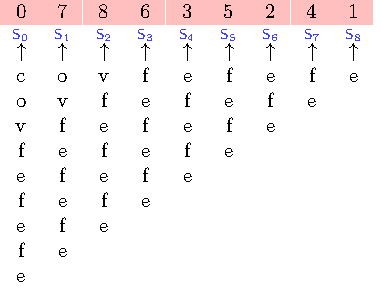
\includegraphics{kapitel/saca_algorithmen/bpr/algorithmus/phase2/bptr_final/image.pdf}
	}
	\caption[Sortiertes Suffix-Array und zugehörige Bucket-Pointer]{Sortiertes Suffix-Array (links) und zugehörige Bucket-Pointer (rechts)}
	\label{fig:buckets_final}
\end{figure}
Bei der Wahl des Sortierverfahrens unterscheidet \bpr abhängig von der Größe eines Buckets zwischen \emph{Insertionsort} und \emph{Quicksort}. Für Buckets mit maximal 15 Elementen wird \emph{Insertionsort} verwendet, während alle größeren Buckets mit einer Variante von \emph{Quicksort} sortiert werden. Ergänzend zur Partitionierung des Buckets in zwei Hälften werden alle an das Pivotelement angrenzenden Elemente mit gleichem Sortierschlüssel von den rekursiv zu sortierenden Partitionen ausgenommen, solange bis in beide Richtungen das erste Element mit unterschiedlichem Schlüssel gefunden wird. Diese Heuristik sorgt dafür, dass je nach Struktur des Eingabestrings die zu sortierenden Partitionen deutlich verkleinert werden können, falls in einem Bucket viele Suffixe den gleichen Schlüssel haben.\par\smallskip
Falls es aufgrund der Struktur des Eingabestrings vorkommt, dass innerhalb eines Buckets alle Suffixe einen gemeinsamen Präfix einer deutlich größeren Länge als \offset haben, dann würde \emph{Quicksort} (bzw. bei kleinen Buckets \emph{Insertionsort}) für mehrere Schritte in der Rekursion versuchen, ausschließlich Elemente mit gleichem Schlüssel zu sortierten. Dies beeinflusst zwar nicht die Korrektheit des Verfahrens, allerdings entsteht durch jeden überflüssigen Sortiervorgang ein unerwünschter und vermeidbarer Aufwand. Um dem entgegen zu wirken, wird eine Heuristik verwendet, welche nach einem \glqq erfolglosen\grqq{} Sortiervorgang die Länge des längsten gemeinsamen Präfixes aller Suffixe in diesem Bucket bestimmt. Der darauf folgende Rekursionsschritt wird dann mit dieser Länge anstelle von \offset aufgerufen.
